Classic tight-binding question with graphene.

\begin{parts}
	\part Sketch of the direct lattice:
	\begin{figure}[H]
		\centering
		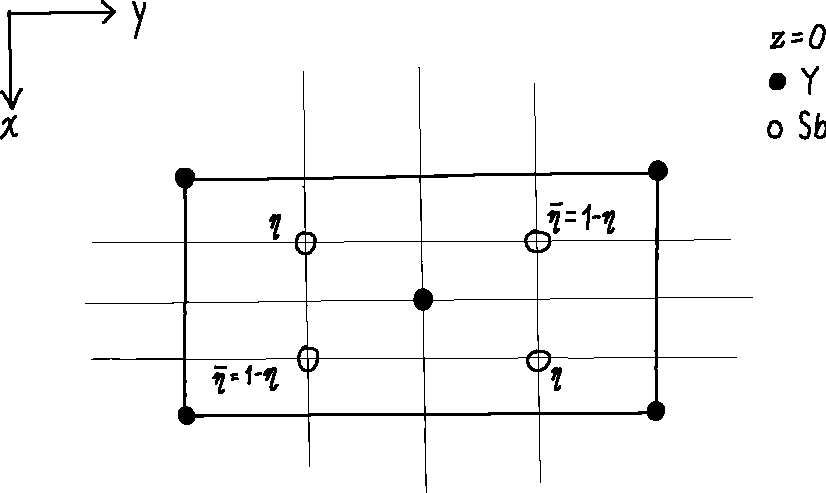
\includegraphics[width=.7\linewidth]{q1-direct-lattice}
	\end{figure}
	
	First we note the relation between $a$ and $a_\textnormal{CC}$:
	\begin{figure}[H]
		\centering
		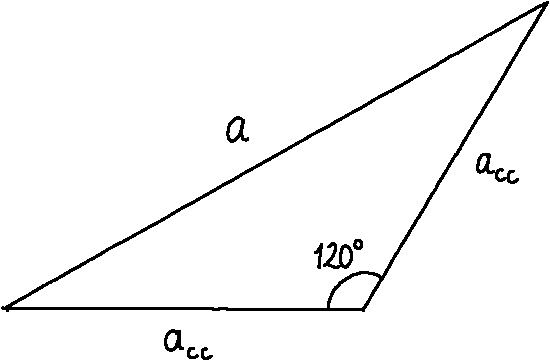
\includegraphics[width=.3\linewidth]{q1-a-acc}
	\end{figure}
	From the diagram, it is clear that $\dfrac{a}{\sin 120\degree} = \dfrac{a_\textnormal{CC}}{\sin 30\degree} \Rightarrow a_\textnormal{CC} = \dfrac{a}{\sqrt{3}}$.
	
	For each type, the nearest neighbours have relative positions:
	\begin{align*}
		\left(a_\textnormal{CC}, 0\right) &= \left(\frac{a}{\sqrt{3}}, 0\right) \\
		\left(-\frac{a_\textnormal{CC}}{2}, \frac{a}{2}\right) &= \left(-\frac{a}{2\sqrt{3}}, \frac{a}{2}\right) \\
		\left(-\frac{a_\textnormal{CC}}{2}, -\frac{a}{2}\right) &= \left(-\frac{a}{2\sqrt{3}}, -\frac{a}{2}\right)
	\end{align*}
	
	\part In the tight-binding model, we begin with the Hamiltonian for the $i$th atom:
	\begin{equation*}
		\mathcal{H}_i = H_\textnormal{at} + \Delta V
	\end{equation*}
	where $H_\textnormal{at} = p_i^2 / 2m + V_i (\mathbf{r})$ is the atomic Hamiltonian, $\Delta V = \sum_{j \neq i} V_j (\mathbf{r})$ is the potential from other atoms.
	
	Next we consider the LCAO as the trial wavefunction:
	\begin{equation*}
		\Psi = \underbracket{\sum_{i=1}^{N}}_{\substack{\textnormal{sum over} \\ \textnormal{lattice}}}
		\underbracket{\sum_{l \in \nu}}_{\substack{\textnormal{sum over} \\ \textnormal{orbitals}}}
		\underbracket{\sum_{d=1}^{M}}_{\substack{\textnormal{sum over} \\ \textnormal{basis}}}
		\underbracket{\alpha_{ild}}_{\substack{\textnormal{normalisation} \\ \textnormal{constant}}}
		\underbracket{\mathrm{e}^{i\mathbf{k}\cdot(\mathbf{R}_i + \mathbf{d}_d)}}_{\textnormal{Bloch wavevector}}
		\underbracket{\phi_{ld}(\mathbf{r} - \mathbf{R}_i)}_{\substack{\textnormal{standalone} \\ \textnormal{atomic wavefunction}}}
	\end{equation*}
	
	For nearest neighbours, we have:
	\begin{equation*}
		\Psi = \alpha_\textnormal{A} \Phi_\textnormal{A} + \alpha_\textnormal{B} \Phi_\textnormal{B}
	\end{equation*}
	where $\alpha_{i} = 1/\sqrt{N}$, $\Phi_{\alpha} = \sum_{i=1}^{N} \mathrm{e}^{i\mathbf{k}\cdot(\mathbf{R}_i + \mathbf{d}_\alpha)} \Phi_\alpha (\mathbf{r} - \mathbf{R}_i)$.
	
	\part Substituting such wavefunction into TISE then gives:
	\begin{gather*}
		\bra{\Psi}\mathcal{H}\ket{\Psi} = \bra{\Psi}E\ket{\Psi} \\
		\Rightarrow \bra{\Psi}H_\textnormal{at}\ket{\Psi} + \bra{\Psi}\Delta V\ket{\Psi} = E \textnormal{\hspace{1em}assuming $\Phi_\textnormal{A}$, $\Phi_\textnormal{B}$ are orthonormal} \\
		= \sum_{a=1}^{N} \sum_{b=1}^{N} \int \mathrm{d}\mathbf{r} \phi_i^* \left(\mathbf{r} - \mathbf{R}_a + \mathbf{d}_i\right) \Delta V \phi_j \left(\mathbf{r} - \mathbf{R}_b + \mathbf{d}_j\right) \cdot \mathrm{e}^{i\mathbf{k}\cdot\left(-\mathbf{R}_a - \mathbf{d}_i + \mathbf{R}_b + \mathbf{d}_j\right)} \\
		= \sum_{\substack{\textnormal{nearest} \\ \textnormal{neighbour}}} \mathrm{e}^{i\mathbf{k}\cdot\left(\mathbf{R}_\textnormal{nn} + \mathbf{d}_{ij}\right)} \underbracket{\int \mathrm{d}\mathbf{r}^\prime \phi_i^* \left(\mathbf{r}^\prime\right) \Delta V \phi_j \left(\mathbf{r}^\prime - \mathbf{R}_\textnormal{nn} + \mathbf{d}_{ij}\right)}_{\tilde{t}_{ij}}
	\end{gather*}
	
	For nearest neighbours we then have:
	\begin{equation*}
		t_{ij} = \left[\mathrm{e}^{i\mathbf{k}\cdot(a/\sqrt{3}, 0)} + \mathrm{e}^{i\mathbf{k}\cdot(-a/2\sqrt{3}, a/2)} + \mathrm{e}^{i\mathbf{k}\cdot(-a/2\sqrt{3}, -a/2)}\right] \underbracket{\tilde{t}_{ij}}_{\substack{\begin{pmatrix}
				0 & t \\ t & 0
		\end{pmatrix} \\ \textnormal{where $t$ is the hopping integral}}}
	\end{equation*}
	
	Hence:
	\begin{equation*}
		t_{ij} = \underbracket{\left[\mathrm{e}^{ik_x \cdot a/\sqrt{3}} + \mathrm{e}^{ik_x \left(-a/2\sqrt{3}\right) \cdot 2\cos\left(k_y \cdot a/2\right)}\right]}_{\gamma} \tilde{t}_{ij}
	\end{equation*}
	
	Now we seek the eigenvalues of the matrix above:
	\begin{align*}
		\textnormal{det}\left[\left(E_0 - E\right)\mathds{1} + t_{ij}\right] &= 0 \\
		\begin{vmatrix}
			E_0 - E & \gamma t \\
			\gamma^* t^* & E_0 - E
		\end{vmatrix} &= 0 \\
		\Rightarrow E &= E_0 \pm \left|\gamma\right| t \textnormal{\hspace{1em}where $E_0$ is the unperturbed energy per atomic site}
	\end{align*}
	
	Now:
	\begin{align*}
		\left|\gamma\right|^2 &= \left(\mathrm{e}^{ik_x \cdot a/\sqrt{3}} + \mathrm{e}^{-ik_x a/2\sqrt{3}} \cdot 2\cos\left(k_y \cdot a/2\right)\right) \left(\mathrm{e}^{-ik_x \cdot a/\sqrt{3}} + \mathrm{e}^{ik_x a/2\sqrt{3}} \cdot 2\cos\left(k_y \cdot a/2\right)\right) \\
		&= 1 + 4\cos^2 \left(\frac{k_y a}{2}\right) + 2\cos\left(\frac{k_y a}{2}\right) \underbracket{\left[\mathrm{e}^{ik_x 3a/2\sqrt{3}} + \mathrm{e}^{-ik_x 3a/2\sqrt{3}}\right]}_{2\cos\left(\sqrt{3}k_x a/2\right)} \\
		&= 1 + 4 \cos\left(\frac{\sqrt{3}k_x a}{2}\right) \cos\left(\frac{k_y a}{2}\right) + 4 \cos^2 \left(\frac{k_y a}{2}\right)
	\end{align*}
	
	Thus recovering the shown dispersion in the question.
	
	We then have the following reciprocal lattice:
	\begin{figure}[H]
		\centering
		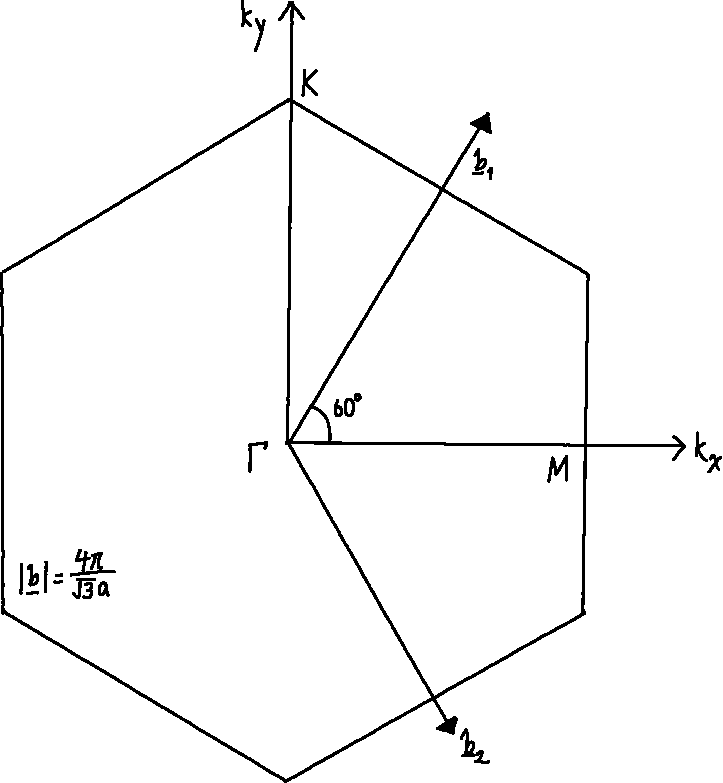
\includegraphics{q1-reciprocal-lattice}
	\end{figure}
	
	With $\kappa$ being a path parameter, we have the following dispersions:
	
	$M$ $\rightarrow$ $\Gamma$: choose path $k_x = \kappa$, $k_y =0$, $\kappa\in\left[2\pi / \sqrt{3}a, 0\right]$:
	\begin{gather*}
		E \simeq E_1 \pm t \sqrt{5 + 4\cos \left(\frac{\sqrt{3}\kappa a}{2}\right)} \\
		\Rightarrow E(M) = E_1 \pm t \qquad E(\Gamma) = E_1 \pm 3t
	\end{gather*}
	
	$\Gamma$ $\rightarrow$ $K$: choose path $k_x = 0$, $k_y = \kappa$, $\kappa\in\left[0, 4\pi / 3a\right]$:
	\begin{gather*}
		E \simeq E_1 \pm t \underbracket{\sqrt{1 + 4\cos\left(\frac{\kappa a}{2}\right) + 4\cos^2 \left(\frac{\kappa a}{2}\right)}}_{2\cos\left(\kappa a/2\right) + 1} \\
		\Rightarrow E(K) = E_1
	\end{gather*}
	
	$K$ $\rightarrow$ $M$: choose path $k_x = 2\pi / \sqrt{3}a$, $k_y = \kappa$, $\kappa\in\left[2\pi / 3a, 0\right]$:
	\begin{equation*}
		E \simeq E_1 \pm t \underbracket{\sqrt{1 - 4\cos\left(\frac{\kappa a}{2}\right) + 4\cos^2 \left(\frac{\kappa a}{2}\right)}}_{2\cos\left(\kappa a/2\right) - 1}
	\end{equation*}
	
	Sketch of graphene dispersion:
	\begin{figure}[H]
		\centering
		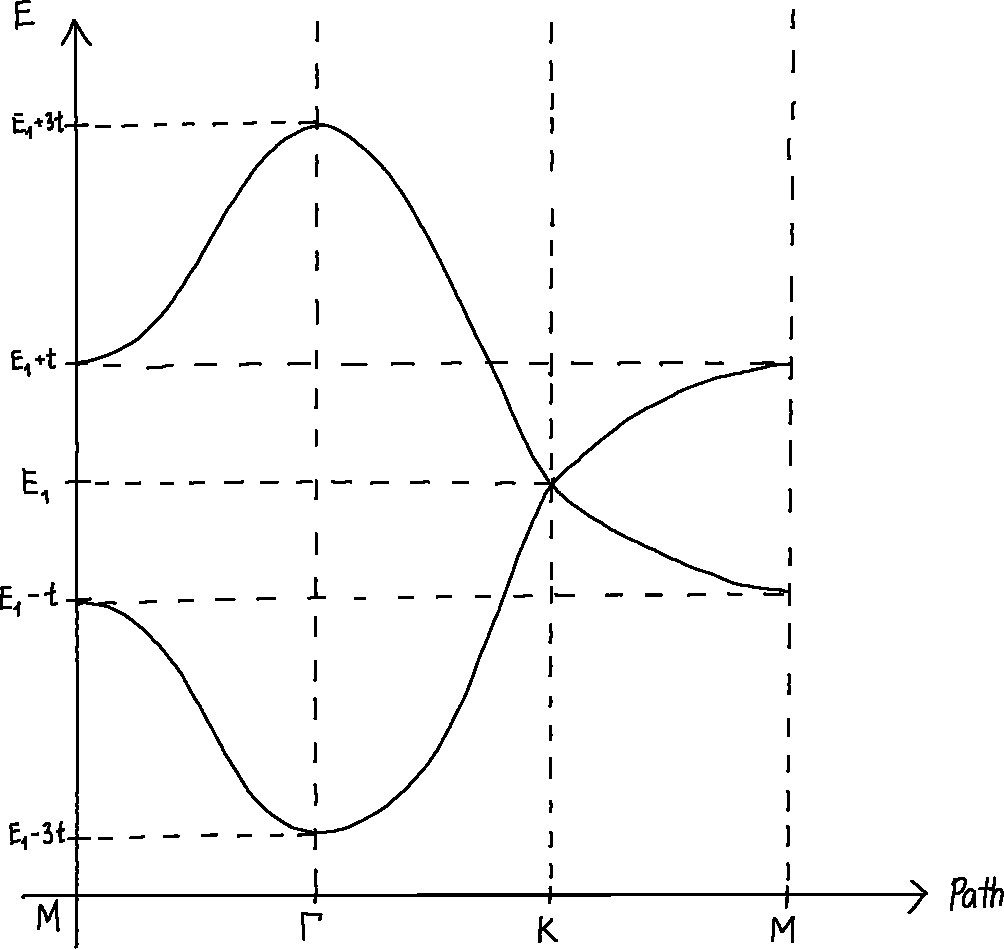
\includegraphics[width=.6\linewidth]{q1-dispersion}
	\end{figure}
	
	As the Fermi energy of graphene is near the Dirac point, its properties will be determined by the dispersion around it -- linear dispersion, conductance...
	
	\part Carbon nanotubes are rolled up along the chiral vector, $\mathbf{n} = n_1 \mathbf{a}_1 + n_2 \mathbf{a}_2$ where $n_i$ are the chiral indices.
	
	Due to the perfect von-Karman boundary conditions, the wavevector along $\mathbf{n}$ is quantised, leaving the perpendicular wavevector quasi-continuous.
	
	\begin{figure}[H]
		\centering
		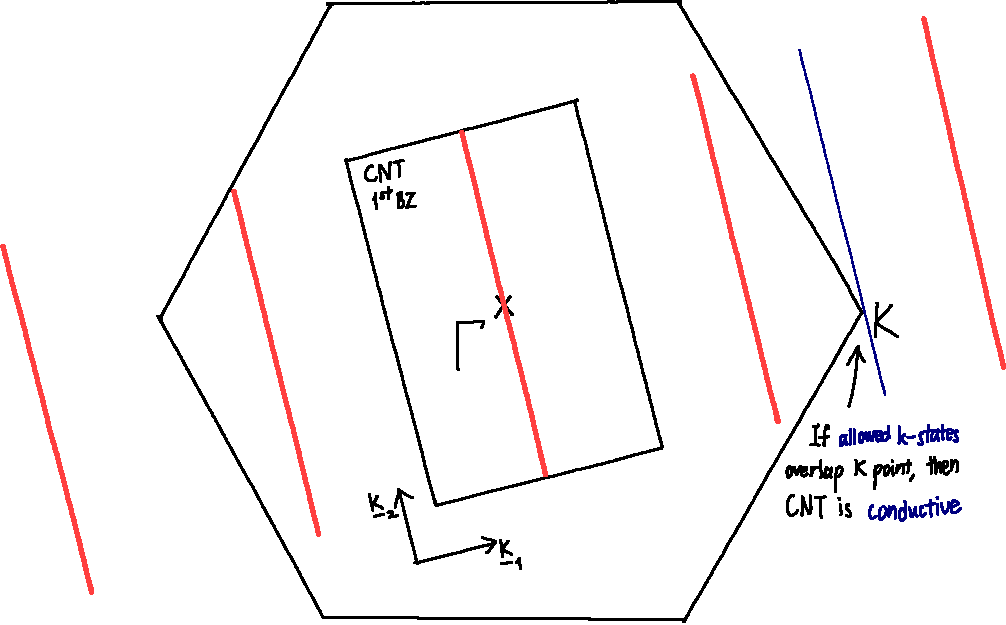
\includegraphics[width=.7\linewidth]{q1-cnt}
	\end{figure}
	As illustrated in the sketch, the allowed energy is then restricted by the locus of allowed $k$ states.
	In particular if such locus overlaps the K point, the nanotube will be conductive.
\end{parts}